\subsection{Strategy results}
\label{sec:results_strategy}

Table \ref{table:financial_metrics} shows the results of the benchmark and the
strategy under test. We can see that the estimate on the Sharpe Ratio is bigger
for benchmark than the strategy under test. Later, evaluation of the
Probabilistic Sharpe Ratio will be used to analyze the confidence on the Sharpe
Ratio estimation for different reference values. Sortino ratio is bigger for the
strategy under test which is aligned with the win loss ratio observation. There
are no considerable differences in other indexes with the exception of the
volatility which has a rough difference of two magnitude orders.

Two indices were not computed for the benchmark strategy: correlation to
underlying (because it would be equal to 1) and the return on execution cost.
The latter will just add noise because only two trades will be executed: one at
the start of the time series and one at the end. Finally, because of the low
observed correlation value we can state that both strategies are doing quite
different things.

\begin{table}[H]
  \centering
  \begin{tabular}{| c | c | c |} 
    \hline
    \multicolumn{3}{|c|}{Financial metrics} \\
    \hline
    Metric & Buy and hold & Strategy under test \\
    \hline
    Sharpe ratio & 2.2156 & 1.2289 \\
    \hline
    Sortino ratio & 2.9138 & 5.7169 \\
    \hline
    Win loss ratio & 1.1171 & 8.0973 \\
    \hline
    Win rate & 0.5637 & 0.5833 \\
    \hline
    Average return & 0.0073 & 0.0065 \\
    \hline 
    Volatility & 1.2062 & 0.0352 \\
    \hline
    Correlation to underlying &  - & 0.0454 \\
    \hline
    Return on execution costs & - & 21.2264 \\
    \hline
  \end{tabular}
  \caption{Financial metrics benchmark.}
  \label{table:financial_metrics}
\end{table}

\begin{figure}[H]
    \centering
    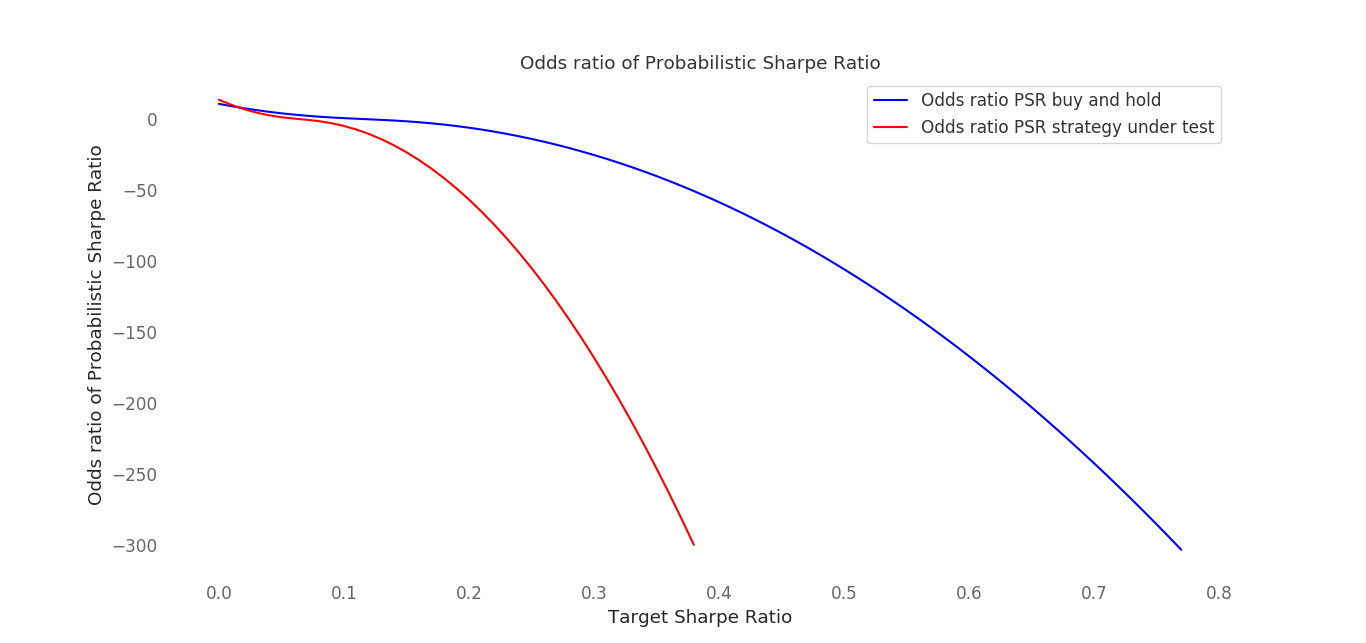
\includegraphics[width=\textwidth]{results/images/log_odds_ratio_psr.png}
    \caption{Odds ratio for the Probabilistic Sharpe Ratio of the buy and hold strategy and the strategy under test.}
    \label{fig:prob_sharpe_ratio}
\end{figure}

Because the Probabilistic Sharpe Ratio is compared against a sequence of target
Sharpe Ratios (0.01 increments between 0. and 1.), it is better shown in terms
log-odds ratio of the PSR values in figure \ref{fig:prob_sharpe_ratio}. It is observed
that for both strategies the odds quickly drop to quite low values below Sharpe
Ratios above 0.1. This is explained by analyzing the Probabilistic Sharpe Ratio
equation (\ref{eqn:prob_sharpe_ratio}). The denominator of the test statistic,
i.e. the standard error, is simply great because of the extremely large kurtosis
and skewness coefficients that both strategies exhibit. See table \ref{table:return_moments}
and remember that the normal distribution has a skewness of 0 and a kurtosis
of 3. Together with the table, figures
\ref{fig:b_h_return_distribution} and \ref{fig:st_return_distribution} display
histograms for the return distributions.

\begin{table}[H]
  \centering
  \begin{tabular}{| c | c | c |} 
    \hline
    \multicolumn{3}{|c|}{Moments of returns} \\
    \hline
    Metric & Buy and hold & Strategy under test \\
    \hline
    Mean of returns & 0.0073 & 0.0065 \\
    \hline
    Variance of returns & 0.0039 & 3.4018 . $10^{-6}$ \\
    \hline
    Skewness of returns & 0.2973 & 19.1115 \\
    \hline
    Kurtosis of returns & 11.9335 & 450.5218 \\
    \hline
  \end{tabular}
  \caption{Moments of the returns for both strategies}
  \label{table:return_moments}
\end{table}

\begin{figure}[H]
    \centering
    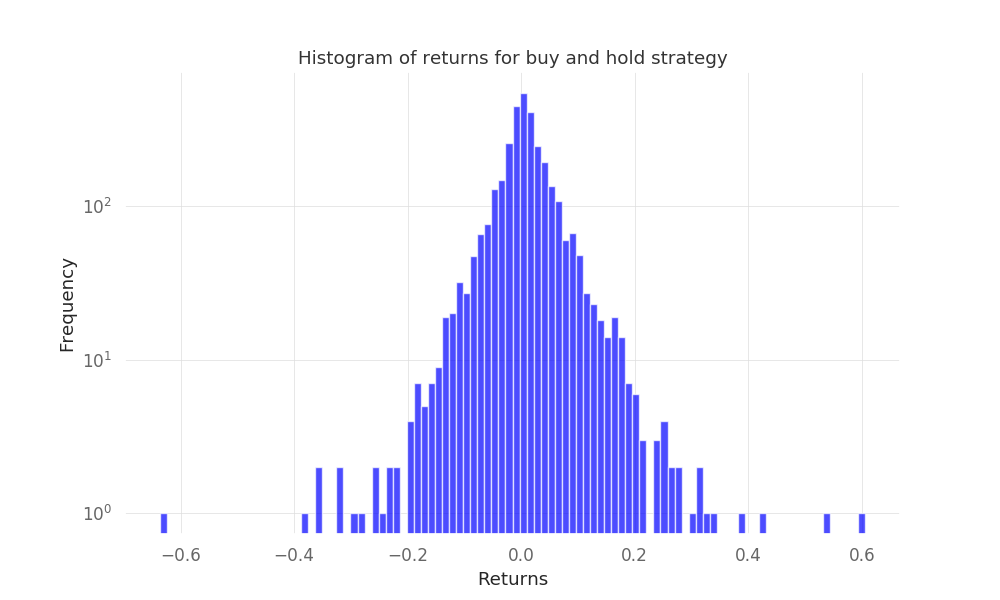
\includegraphics[width=1.1\textwidth]{results/images/hist_returns_btc.png}
    \caption{Buy and hold return distribution.}
    \label{fig:b_h_return_distribution}
\end{figure}

\begin{figure}[H]
    \centering
    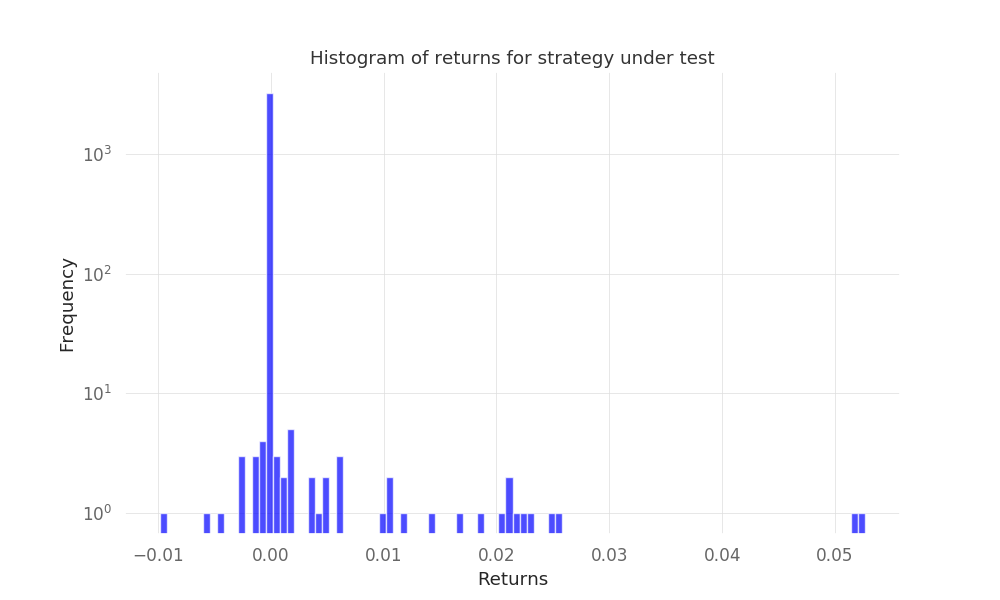
\includegraphics[width=1.1\textwidth]{results/images/hist_returns_st.png}
    \caption{Strategy under test return distribution.}
    \label{fig:st_return_distribution}
\end{figure}
